\documentclass[
% -- opções da classe memoir --
12pt,				% tamanho da fonte
openright,			% capítulos começam em pág ímpar (insere página vazia caso preciso)
twoside,			% para impressão em frente e verso. Oposto a oneside
a4paper,			% tamanho do papel. 
% -- opções da classe abntex2 --
%chapter=TITLE,		% títulos de capítulos convertidos em letras maiúsculas
%section=TITLE,		% títulos de seções convertidos em letras maiúsculas
%subsection=TITLE,	% títulos de subseções convertidos em letras maiúsculas
sumario=tradicional, % configura estilo do sumário (comente estilo ABNTEX)
%subsubsection=TITLE,% títulos de subsubseções convertidos em letras maiúsculas
% -- opções da classe hyperref
hidelinks,          % oculta caixas e links coloridos
% -- opção de numerar continuamente as equações
%continuouseq,      % descomente para numeração contínua
% -- opção para citações e referências padrão IEEE	
%IEEE,				% citações e referências IEEE
% -- opções para citação utilizando classe abnt2cite
%alf,				% citação alfanumérica
num,				% citação numérica 
%overcite,			% citação no modo sobrescrito (se usar notas de rodapé, evite)
bibjustif,			% alinhamento justificado para as referências
brackets,			% citações com delimitador []
% -- opções do pacote babel --
english,			% idioma adicional para hifenização
brazil				% o último idioma é o principal do documento
]{article}       % utfprcopel.cls based on abnt2.cls


\usepackage{sbc-template}
\usepackage{float}
\usepackage{graphicx,url}
\usepackage{verbatim}                                       % Permite apresentar texto tal como escrito no documento, ainda que sejam comandos Latex
\usepackage{amsfonts, amssymb, amsmath}                     % Fontes e símbolos matemáticos
\usepackage{ae, aecompl}                                    % Fontes de alta qualidade
\usepackage{latexsym}                                       % Símbolos matemáticos
\usepackage[algoruled, portuguese]{algorithm2e}             % Permite escrever algoritmos em português
\usepackage[brazil]{babel}
\usepackage[utf8]{inputenc} 
\usepackage{indentfirst}
\usepackage{listings}
\usepackage{color}

\definecolor{dkgreen}{rgb}{0,0.6,0}
\definecolor{gray}{rgb}{0.5,0.5,0.5}
\definecolor{mauve}{rgb}{0.58,0,0.82}

\lstset{frame=tb,
  language=C,
  aboveskip=3mm,
  belowskip=3mm,
  showstringspaces=false,
  columns=flexible,
  basicstyle={\small\ttfamily},
  numbers=none,
  numberstyle=\tiny\color{gray},
  keywordstyle=\color{blue},
  commentstyle=\color{dkgreen},
  stringstyle=\color{mauve},
  breaklines=true,
  breakatwhitespace=true,
  tabsize=3
}
\renewcommand{\lstlistingname}{Código}% Listing -> Algorithm
\sloppy

\title{Obtenção de sequências aleatórias a partir de interferência eletromagnetica}

\author{Cristiano M. Matsui\inst{1}, Kallil M. Caparroz\inst{2}, Rodrigo C. Anater\inst{3} }


\address{Universidade Tecnológica Federal do Paraná - Câmpus Pato Branco
  \email{cristiano.matsui@gmail.com, kallil@alunos.utfpr.edu.br,
  rodrigoanater@alunos.utfpr.edu.br}
}

\begin{document} 

  \selectlanguage{brazil}
  \maketitle

\begin{abstract} 	
 	The definition of what is meant by a random number or event is the subject of discussion by professionals in many fields of study, including computing professionals. However, most part of the computers used in the present days generate only pseudorandom numbers. This article details the development of a random number generator using the electrical noise obtained from the analog port of a microcontroller
\end{abstract}
     
\begin{resumo} 
 	A definição do que se entende por um número ou evento aleatório é alvo de debates por parte de profissionais de diversas áreas de estudo, inclusive profissionais de computação. Entretanto, a maioria dos computadores presentes na atualidade geram apenas números pseudo-aleatórios. O presente artigo detalha o desenvolvimento de um gerador de números aleatórios utilizando o ruído elétrico obtido da porta analógica de um microconrolador.  
\end{resumo}


\section{Introdução}
\section{Geração de Sequências Aleatórias}
Em geral, sistemas computacionais são determinísticos, ou seja, cada evento é definido pela sequência de eventos precedentes. Essa é basicamente a definição contrária à definição de aleatoriedade, criando assim um problema na geração de números aleatórios por computadores. Porém, existem duas maneiras principais de se resolver esse problema.
Uma forma é a utilização de sequências pseudoaleatórias. Essas sequências se baseiam em uma série de operações determinísticas que, a partir de um conjunto de parâmetros, são capazes de gerar sequências que se pareçam suficientemente aleatórias para alguma finalidade específica. Esse método tem algumas vantagens, como uma grande eficiência, gerando grandes sequências em um curto período de tempo, e reprodutibilidade, que permite a repetição de testes, uma vez que o mesmo conjunto de parâmetros iniciais gera a mesma sequência.

Porém, em muitos casos, como para criptografia, a reprodutibilidade dos dados não é desejada, pois os valores devem ser realmente imprevisíveis. Para tal, existem os chamados geradores de números verdadeiramente aleatórios, que devido à natureza determinística de sistemas computacionais, necessitam de obtenção de dados externos ao computador.
 
É comum geradores pseudoaleatórios se utilizarem de algum dado externo como parâmetro para a geração de suas sequências, como o tempo do sistema, de forma à variar seus resultados. Já geradores de sequências numéricas verdadeiramente aleatórios, dependem de uma fonte de dados aleatórios para a geração da sequência, dados estes que devem apresentar alguma forma de aleatoriedade intrínseca. Assim, geradores de números verdadeiramente aleatórios costumam se utilizar da medição de fenômenos físicos, como sons atmosféricos ou até mesmo decaimento radioativo.

\section{Materiais e Métodos}
\subsection{Materiais}
Para captar e realizar a leitura do ruído eletromagnético foram utilizados uma antena para a captação
e um microcontrolador para a aquisição do valor do ruído captado.
\subsubsection{Arduino UNO}
O Arduino Uno (Fig 1) é uma placa de microcontrolador baseado no ATmega328 (datasheet). Possui 14 pinos de entrada/saída digital (dos quais 6 podem ser usados como saídas PWM), 6 entradas analógicas, um cristal oscilador de 16MHz, uma conexão USB e uma entrada de alimentação uma conexão ICSP.

O microcontrolador foi responsável pela leitura do ruído eletromagnético em uma de suas portas analógicas. O ruído foi então convertido para um valor numérico através do conversor analógico-digital (ADC) presente no Arduino.

\begin{figure}[H]
	\label{fig1}
	\begin{centering}
		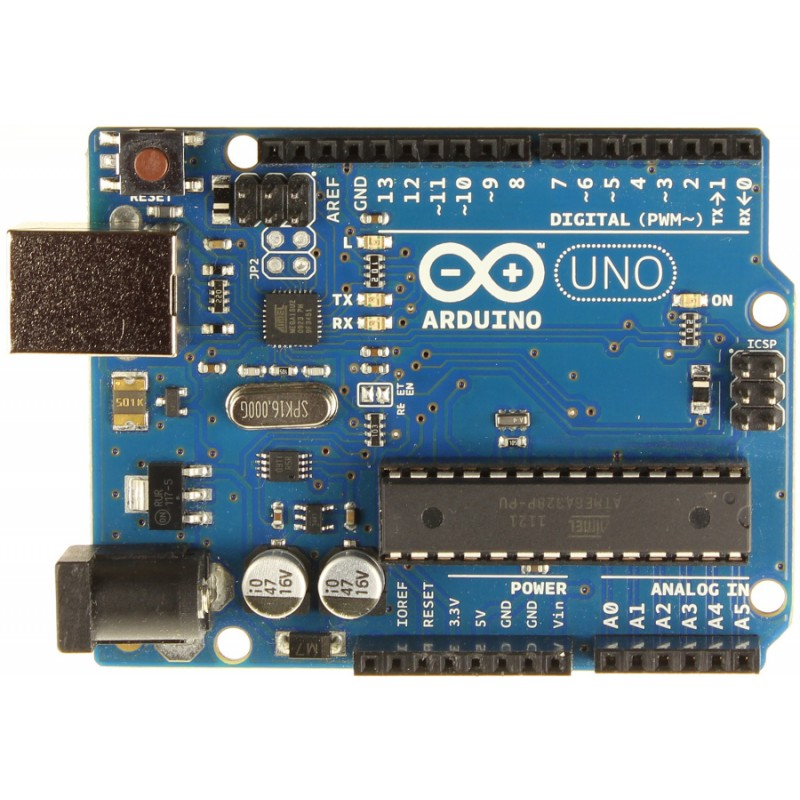
\includegraphics[width = 400pt]{img/arduino.jpg}
		\caption{Arduino UNO}
	\end{centering}	
		
\end{figure}

\subsubsection{Antena}

Foi utilizado um fio de estanho na porta do microcontrolador como aparato para a captação de interferência eletromagnética. A configuração escolhida da antena foi de monopolo de quarto de onda \cite{Balanis2005}.
A frequência captada pela antena é prevista pela equação abaixo:

\begin{equation}
   f = \frac{c}{\frac{L}{4}}
  \end{equation}
sendo $f$ a frequência em Herz, $c$ a velocidade da luz e $L$ o comprimento da antena. Para uma antena de 8 centímetros, a frequência
captada pela antena é de 15MHz.
 \begin{figure}[H]
 	\label{fig2}
 	\begin{centering}
 		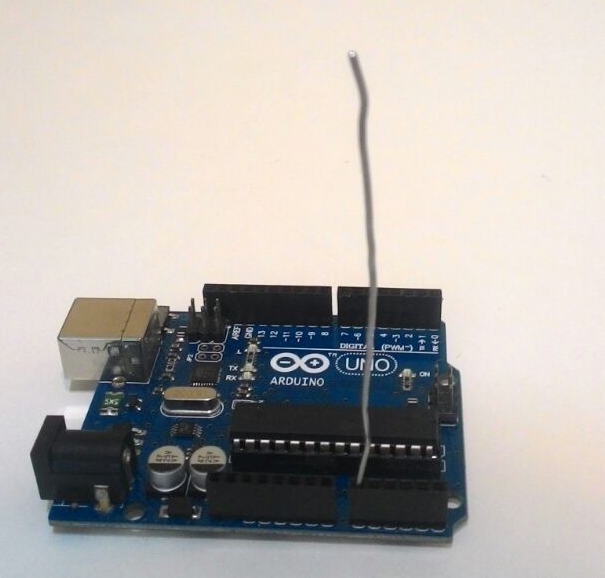
\includegraphics[width = 200pt]{img/arduino2.png}
 		\caption{Arduino UNO com a antena monopolo}
 	\end{centering}	
 		
 \end{figure}

\subsection{Métodos}
\section{Validação dos resultados}
Para avaliar o nível de aleatoriedade das sequências, foi utilizado o programa \textit{ent}, que foi criado com o objetivo de realizar a avaliação de geradores de sequências numéricas pseudoaleatórias para criptografia e aplicações de amostragem estatística. O programa realiza cinco testes diferentes:
\begin{itemize}
\item Entropia: Analisa a densidade de informação apresentada, ou seja, verifica o quanto a sequência pode ser comprimida e ainda representar o dado original. Quanto menor for a entropia, menos aleatória e mais compressível é a sequência.
\item Teste Qui-quadrado: É calculada a distribuição qui-quadrado, que avalia a relação entre os valores fornecidos e os esperados. A distribuição é simétrica, sendo que sequências verdadeiramente aleatórias devem resultar em valores mais centralizados \cite{knuth1998art}. Valores maiores que 99\% ou menores que 1\% são não-aleatórios. Valores entre 99\% - 95\% ou entre 1\% - 5 \% são suspeitos de não serem aleatórios. Valores entre 5\% - 10\% ou entre 95\% - 90\% são quase suspeitos. Qualquer outra faixa de valores valida a sequência como aleatória. 
\item Média Aritmética: Realiza a média aritmética dos valores. Considerando que a analise é feita a partir de blocos de quatro bytes, ou seja, são valores entre zero e 255, idealmente a média deve se aproximar de 127,5. 
\item Aproximação de $\pi$ pelo método de Monte Carlo: Cada sequência sucessiva de seis bytes é utilizada como coordenadas em um quadrado, o qual contem um circulo inscrito. Pontos verdadeiramente aleatórios tem uma probabilidade de estar dentro do circulo igual à razão entre a área do circulo pela área do quadrado. Assim, a razão entre os pontos do circulo e o total de pontos deve tender (lentamente) à um quarto do valor de $\pi$.
\item Coeficiente de correlação serial: Mede o quanto cada elemento da sequência se relaciona ao elemento anterior, e para sequências verdadeiramente aleatórias, deve se aproximar de zero.
\end{itemize}
Deve-se ressaltar, porém, que não existem testes definitivos de aleatoriedade, uma vez que qualquer teste deve-se basear em probabilidades, e não certezas. Dessa forma, é de se esperar que, após realizada uma certa quantidade de testes, uma sequência verdadeiramente aleatória falhe em alguns deles, porém com menor probabilidade de que uma sequência não aleatória
\section{Resultados}

Os arquivos binários obtidos foram submetidos ao programa \textit{ent}, para verificar os cinco testes de aleatoriedade da sequência gerada.
Foram utilizadas cinco sequências geradas pelo experimento, e uma sequência gerada pelo gerador de entropia do sistema GNU/Linux.

\begin{table}[H]
\caption{Verificação da aleatoriedade dos dados}
\centering
\resizebox{\columnwidth}{!}{%
\begin{tabular}{|c|c|c|c|c|c|}
 \textbf{Instância}&\textbf{Entropia}&\textbf{\% Qui-quadrado}&\textbf{Média aritimética}&\textbf{Monte-Carlo}&\textbf{Correlação serial}\\
 seq1& 7.961164  & 25.75 & 126.8750 & 3.236494598& 0.005960 \\
 seq2& 7.969834  & 98.34 & 126.7858 & 3.150060024& 0.016754 \\
 seq3& 7.961094  & 35.11 & 125.8314 & 3.154861945& -0.006693 \\
 seq4& 7.960302  & 19.38 & 126.1190 & 3.164465786& 0.005694 \\
 seq5& 7.952913  & 0.29 & 124.9390 & 3.222088836& 0.007775 \\
 seq\_urandom& 7.965104  & 70.94 & 128.3805 & 3.090269637& 0.021974 \\
 

\end{tabular}
}
\end{table}







\bibliographystyle{sbc}
\bibliography{sbc-template}
\end{document}